\chapter{Entorno Empresarial}
\thispagestyle{empty} % Quitar el número

En este capítulo se describe el entorno empresarial en el cual tuvo lugar el desarrollo del proyecto de pasantía, la empresa Fischer, Knoblauch \& Co (FKC) filial de Frankfurt. Se exponen brevemente su misión y visión  

\section{Fischer, Knoblauch \& Co.}

Es un proveedor de servicios multimedia especializado en el área de aprendizaje electrónico. Esta presente en Frankfurt y Munich en Alemania asi como en Basel, Suiza. Fundada en 1996 por Guy Fischer y Thomas Knoblauch.

Proveen consultoria en la integración y ampliación del aprendizaje electrónico a compañias de diversos sectores en Alemania y Bélgica. Se encargan de sugerir la elecciones de tecnologías, concepción del plan de aprendizaje, didacticas y metódologia de la enseñanza, producción del contenido audiovisual, hasta la integración de la solución en el ambiente del cliente. 

Basicamente, si una compañia quiere enseñar una cierta habilidad a sus empleados contacta a un proveedor de servicios de aprendizaje electrónico, FKC en este caso, los ayuda a integrar un plan aprendizaje a su empresa, que se ven materializados en entrenamientos basados en la web. 



\section{Estructura organizacional}

En la Figura se muestra la estructura organizacional de FKC Frankfurt:

\begin{figure}[h]
\begin{center}
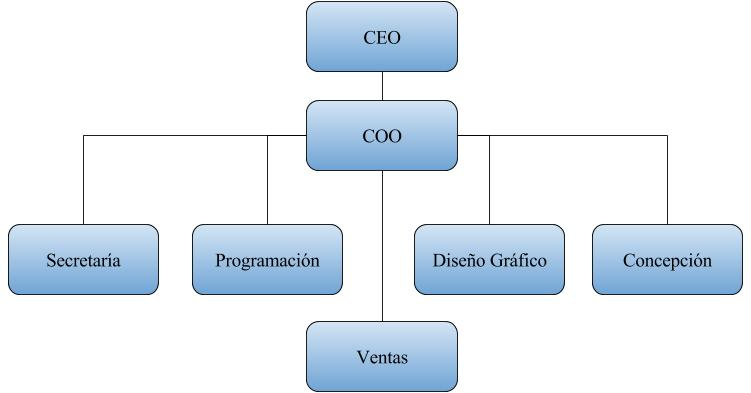
\includegraphics{figuras/estructuraFKC.jpg}
\end{center}
\end{figure}
